\rhead{实验与结果分析}
\chapter{实验与结果分析}

%@@@@@@@@@@@@@@@@@@@@@@@@@@@@
\section{数据集及预处理}
实验所用的所有数据均来自Isobase数据库\cite{park2011isobase}。该数据包含了四种生物的PPI网络数据,每种生物的PPI网络详细信息见表\ref{table:1}。表中的数据是经过预处理的,其中每个PPI网络去除了自环、重边以及独立的节点。Isobase数据库是被普遍使用的生物PPI网络数据库,因此我们选择了这个数据集。


\begin{table}[htbp]
    \centering
    \caption{Isobase数据库关于四种生物的PPI网络数据}
    \label{table:1}
    \begin{tabular}{cccc}
         \hline 物种&点数&边数&平均点度\\
         \hline C.elegans&2974&4827&3.25\\
         D.melanogaster&7387&24937&6.75\\
         H.sapiens&\bf{10296}&54654&10.62\\
         S.cerevisiae&5523&\bf{82656}&\bf{29.93}\\
         \hline
    \end{tabular}
\end{table}

这些都是静态的PPI网络数据,为了构造动态的PPI网络数据,本文使用\cite{zhang2016method}同本文所结合的的方法,对每个PPI网络各生成了一个动态PPI网络。为了叙述方便,对这四种生物我们简单的以ce,dm,hs,sc来称呼它们。

%@@@@@@@@@@@@@@@@@@@@@@@@@@@@@@@@@
\section{实验方法与环境}
除了本文提出的SGOPT算法,本文还使用了全局比对算法中的四种经典算法作为和本文算法的对比,分别是IsoRank\cite{singh2008global},SPINAL\cite{aladaug2013spinal},L-GRAAL\cite{malod2015graal}和PROPER\cite{kazemi2016proper}算法。SGOPT算法全部代码由Java构成,并且运行在Linux Ubuntu环境下,详细的环境参数见表\ref{table:2}。

\begin{table}[htbp]
    \centering
    \caption{实验运行环境}
    \label{table:2}
    \begin{tabular}{l|l}
         \hline 
         CPU&Intel Core i7-4790K, 4.00GHz\\
         \hline
         内存&16G\\
         \hline
         操作系统&Linux Ubuntu 14.04LTS,64位\\
         \hline
    \end{tabular}
\end{table}

关于实验中用到的比对衡量标准,CE指标是我们首要衡量的指标。其次,我们也要衡量DEC,DICS,$DS^3$和DTWEC这四个指标。

%@@@@@@@@@@@@@@@@@@@@@@@@@@@@@@@@@@@@@
\section{关于SGOPT算法的$\alpha,\beta$参数的选择}

正如前文所说的,$\alpha,\beta$作为SGOPT算法的重要参数,太小了可能会导致实验结果变差,太大了则会导致算法耗时,该如何选择一组优秀的参数呢?本文采取了实验确定的办法。

为了描述方便,我们用生物名称1-生物名称2的形式来代表对生物1和生物2的PPI网络进行比对的一组实验,即比对生物1的静态PPI网络和生物2的动态PPI网络,例如ce-dm就是比对ce的静态PPI网络与dm的动态PPI网络,以此类推。

首先我们来确定参数$\beta$。

参数$\beta$影响的是每次删掉的匹配点对数,因此$\beta$越大,删掉的匹配点对数便越多,二分图便越大,导致一次迭代的时间就越长。但是,$\beta$对比对效果的影响如何呢?我们希望挑选在同样的时间下,能够产生更好比对效果的$\beta$参数。因此,我们先给$\alpha$设定一个很大的值,让SGOPT算法可以无限迭代,然后我们选择不同的$\beta$值,让SGOPT算法分别跑10秒,20秒,30秒,40秒,50秒,60秒,看看不同的$\beta$参数在同样时间的情况下,产生的比对的效果。之所以采用比较短的运行时间,是因为在长的运行时间下,迭代的过程可能会收敛,产生的比对效果随时间的变化会变得没这么“敏感”,不利于我们观测$\beta$值对比对效果的影响。
\begin{figure}[htbp]
\centering
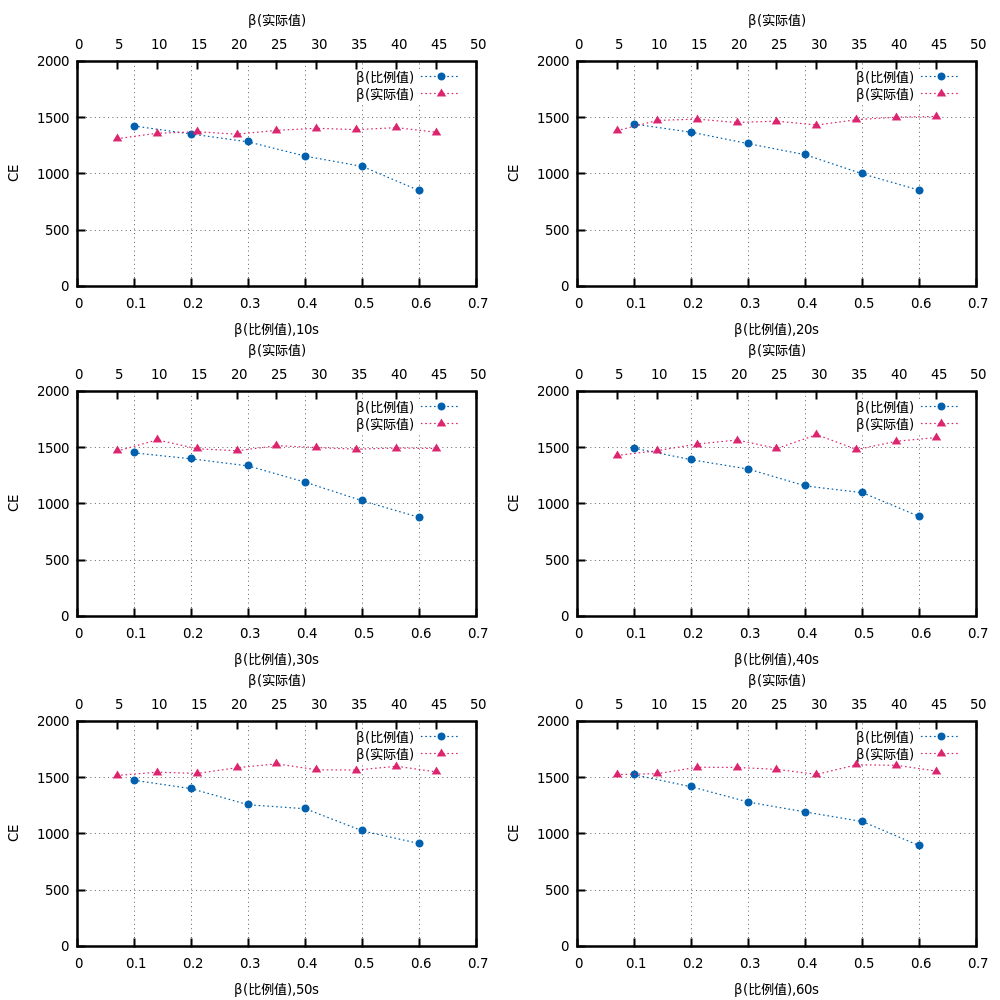
\includegraphics[width=\textwidth]{pic/beta.png}
\caption{SGOPT在不同$\beta$值时运行$10s,20s,30s,40s,50s,60s$的结果} 
\label{fig:beta}
\end{figure}

图\ref{fig:beta}是SGOPT算法在ce-dm实验组中优化IsoRank算法的结果。$\beta$(实际值)的意思就是每次迭代时删除的匹配点对的数目(而不是比例)。蓝色曲线是$\beta$从0.1到0.6变化时SGOPT得到的比对的结果,从中可以看出,过大的$\beta$意味着每次被删掉的匹配点对数比较多,需要调整的匹配点对也越多,一轮的迭代时间会增加,同样的运行时间的情况下,在$\beta$接近0.6的时候,比对效果明显变差,说明SGOPT不适合$\beta$过大的情况。

而红色曲线表明,每轮迭代时,如果删除的匹配点对数比较少,那么SGOPT算法在同样的时间内,都能很快调整出比较优的解,而且在这种情况下$\beta$稍微大点的效果会比较好。因此我们最终选定$\beta=35$作为SGOPT的参数。

其实,$\beta$参数的好坏,只是决定了出同样结果的时间快慢,理论上,任意的$\beta$值,只要有一定的时间,都能够调整出好的解,但是为了更快得到这个解,我们还是希望尽量挑选出更好的$\beta$值。

从SGOPT算法中可以看出,每次迭代,比对的效果不可能变差,所以随着时间的增加,比对的效果只会越来越好。但是随着时间的推移,能找到更优比对的概率变得越来越小,因此整个迭代会有一个"收敛"的过程。而$\alpha$参数是迭代次数,也就是时间长短,我们选择$\beta=35$的情况下来运行SGOPT算法,并且记录每轮迭代后当前比对的CE值。

\begin{figure}[htbp]
\centering
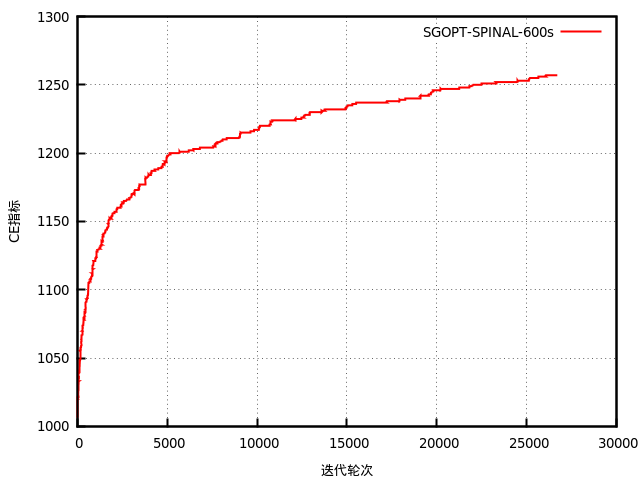
\includegraphics[height=0.4\textheight]{pic/alpha.png}
\caption{SGOPT每轮迭代时的比对结果(CE)} 
\label{fig:alpha}
\end{figure}

图\ref{fig:alpha}是SGOPT算法在$\beta=35$的情况下,在实验组ce-dm上优化IsoRank算法跑了5分钟的的实验结果,可以看到,在前2000轮迭代时,比对的效果变化十分明显,而2000轮之后,比对的效果变化开始趋于平缓,说明算法能够得到更优比对的概率变低了,但是依旧呈上升趋势。

\begin{figure}[htbp]
\centering
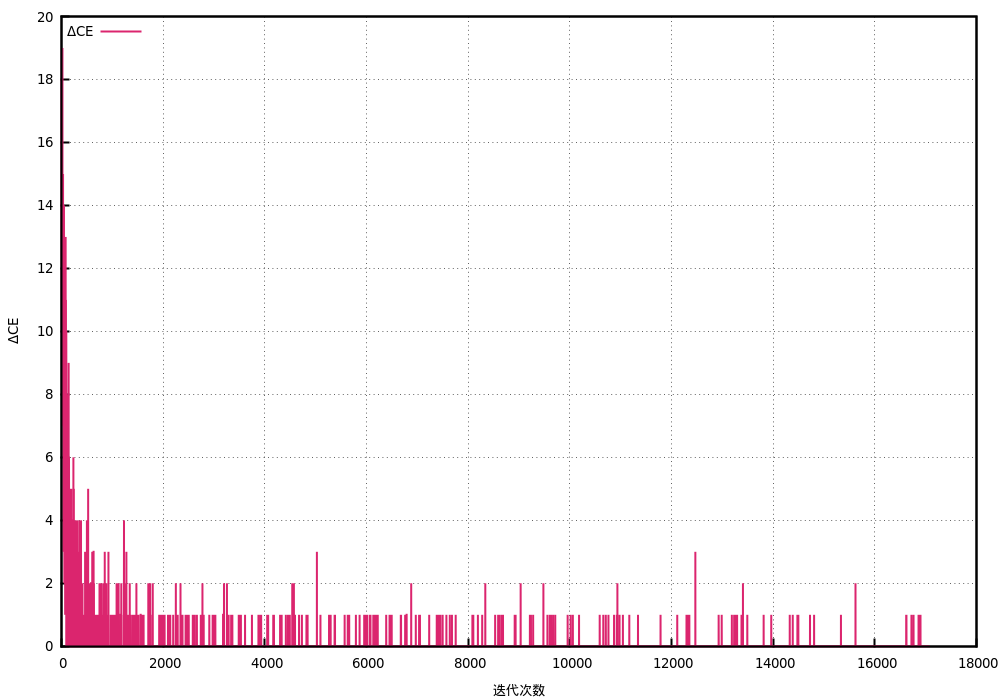
\includegraphics[height=0.4\textheight]{pic/alpha_d.png}
\caption{SGOPT每轮迭代时的比对结果$(\Delta CE)$} 
\label{fig:alpha_d}
\end{figure}

图\ref{fig:alpha_d}是图\ref{fig:alpha}关于$\Delta CE$值(即每次迭代比对效果比之前迭代的比对效果好的量)的实验结果。从中大概可以看出,在迭代2000次以后,每次更新当前最优比对的时候,CE值增幅基本只在1,2跳动,偶尔能够有3的增幅,并且随着迭代次数的增加,这样的增幅机会变得越来越少(空隙越来越大)。最终,我们设定$\alpha=14000$作为之后实验的参数。

而且,结合图\ref{fig:beta}也可以看出,$\beta=35$的情况下,算法运行$60s$之后,CE值就超过了1500,而这正是图\ref{fig:alpha}中大约迭代次数为2000左右的时候。所以SGOPT算法可以大约在1分钟左右就能找比较优的解了。

%@@@@@@@@@@@@@@@@@@@@@@@@@@@@@@@@@@@@@@@@@
\section{不同算法之间的比较}

确定了$\alpha,\beta$参数以后,接下来的实验就是SGOPT算法与其他算法的比较。我们分别做了ce-dm,ce-hs,cs-sc,dm-hs,dm-sc,hs-sc六组实验,每组实验都先用四种静态比对算法,求得初始比对$f$(方案一),然后以$f$为基础比对运行SGOPT算法,最终得到新的比对。同时,每组实验还使用四种静态比对算法在动态PPI网络组成的每个静态PPI网络上作比对(方案二),将得到的结果与SGOPT和方案一进行比较。

四种静态比对算法的运行参数见表\ref{table:3}。

\begin{table}[htbp]
    \centering
    \caption{静态比对算法与运行参数}
    \label{table:3}
    \begin{tabular}{ccc}
         \hline 算法&命令行&参数\\
         \hline IsoRank&-alpha $\alpha$ -I 50&$\alpha=1$\\
         SPINAL&-II -alpha $\alpha$&$\alpha=1$\\
         L-GRAAL&-alpha $\alpha$&$\alpha=1$\\
         PROPER&$-l$ $l$ $-r$ $r$&$l=500,r=1$\\
         \hline
    \end{tabular}
\end{table}

图\ref{fig:all}为SGOPT算法与其他四种静态比对算法在\textbf{方案一}之下的比较结果。横坐标表示实验组,纵坐标是比对结果,可以看出,四种静态算法在动态PPI网络上的比对结果各有好坏,IsoRank的结果是最差的,而L-GRAAL的结果则比起其他三种算法都要好。SPINAL和PROPER则没有明显的效果差别。而SGOPT的柱状图表示,对于已有的四种静态比对算法,SGOPT都能在它们已有的比对上改良它们的比对效果,产生效果更好的比对。从中可以看出SGOPT算法相对于\textbf{方案一}在比对效果上有明显的优势。

值得一提的是,虽然IsoRank在动态PPI网络上的比对效果非常糟糕,但是经过SGOPT改良后的比对,效果甚至高于L-GRAAL经过SGOPT改良后的比对,这可能是因为糟糕的比对给了SGOPT更多调整的机会与空间,使得SGOPT能够从全局的角度上来优化整个比对,从而产生了更优秀的比对结果。

\begin{figure}[htbp]
\centering
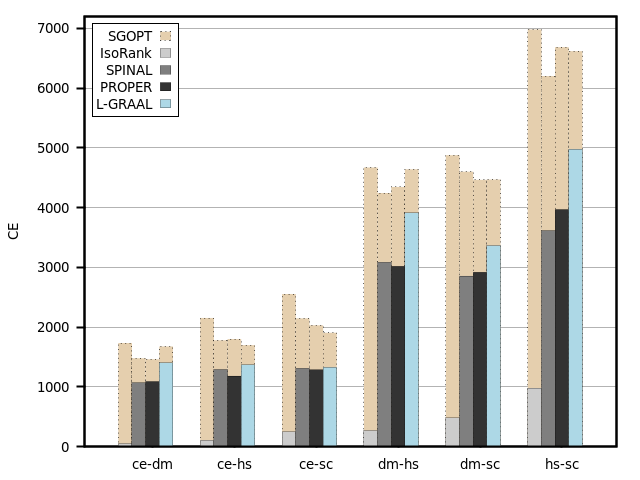
\includegraphics[height=0.25\textheight]{pic/all.png}
\caption{SGOPT与其他四种算法在\textbf{方案一}下的结果比较} 
\label{fig:all}
\end{figure}

\begin{figure}[htbp]
\centering
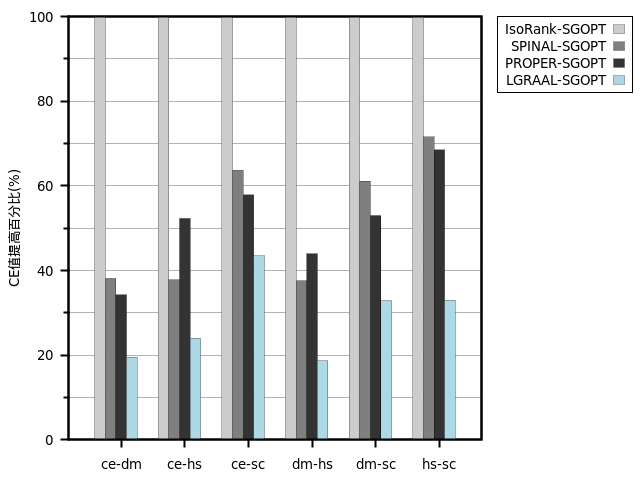
\includegraphics[height=0.25\textheight]{pic/all_improve.png}
\caption{SGOPT相比其他四种算法在\textbf{方案一}下的提高程度} 
\label{fig:all_improve}
\end{figure}

图\ref{fig:all_improve}展示了SGOPT对于其他四种算法在\textbf{方案一}下的效果的提高程度,即
\begin{equation}
\frac{\text{提高后的CE值-提高前的CE值}}{\text{提高前的CE值}}    
\end{equation}
可以看到SGOPT对于提高IsoRank的比对有明显的效果。而对于其他四种算法的提高,SPINAL和PROPER能够达到40\%~60\%,而对于L-GRAAL算法效果的提高则稍微差一点,为20\%~40\%左右。然而总体上来说,有这种结果已经能够充分说明SGOPT相比\textbf{方案一}所具有的优势。

图\ref{fig:all2}为SGOPT算法与其他四种静态算法在\textbf{方案二}之下的比对效果的比较结果。可以看到,除了IsoRank算法,另外的其他三种静态比对算法,在方案二的情况下,都比SGOPT算法好一点。IsoRank算法的效果则显得尤为糟糕,即使是在方案二的情况下。

可见通过逐一和动态PPI网络组成的每一个静态PPI网络进行比对,从中挑选出效果最好的比对的这个方案,在\textbf{比对效果}上,依旧是静态算法比SGOPT算法略胜一筹的。但是正如前文分析的,方案二的最大缺点,则在于时间的极度消耗上。因此,我们需要对方案一,方案二,以及SGOPT算法的运行时间作比较分析,来看看孰优孰劣。

\begin{figure}[htbp]
\centering
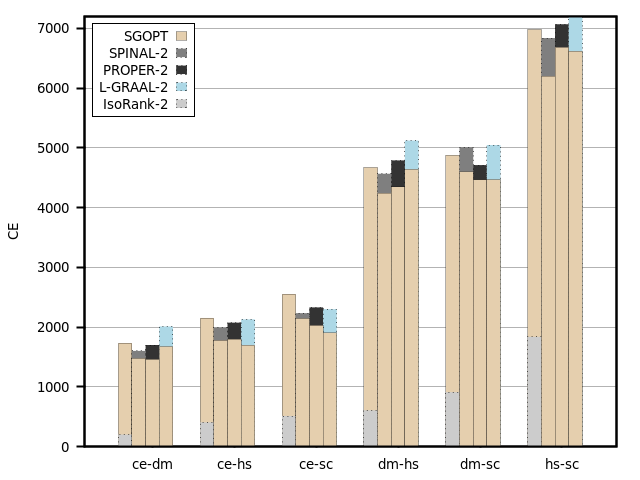
\includegraphics[height=0.25\textheight]{pic/all2.png}
\caption{SGOPT与其他四种算法在\textbf{方案二}下的结果比较} 
\label{fig:all2}
\end{figure}


图\ref{fig:allt}是SGOPT算法与其他四种静态算法在\textbf{方案一}的情况下运行时间的比较结果。由于SGOPT是基于静态算法的,所以SGOPT的运行时间肯定比对应的静态算法长(得先跑一遍静态算法求出比对$f$,SGOPT再以此为基础调整比对)。从中还可以看出,本实验中,L-GRAAL算法的运行时间较长,这是由其运行参数决定的,可以详见表\ref{table:3}。
\begin{figure}[htbp]
\centering
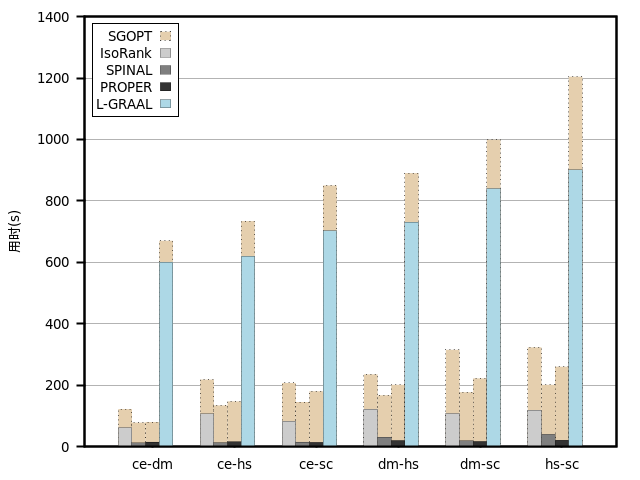
\includegraphics[height=0.25\textheight]{pic/allt.png}
\caption{SGOPT与其他四种算法在\textbf{方案一}下的运行时间比较} 
\label{fig:allt}
\end{figure}

图\ref{fig:allt2}则是SGOPT算法与其他四种静态算法在\textbf{方案二}的情况下运行时间的比较结果。
\begin{figure}[htbp]
\centering
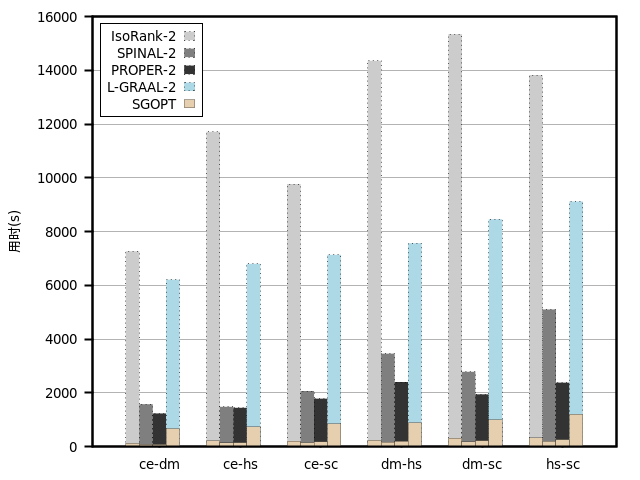
\includegraphics[height=0.25\textheight]{pic/allt2.png}
\caption{SGOPT与其他四种算法在\textbf{方案二}下的运行时间比较} 
\label{fig:allt2}
\end{figure}

为了突出方案一,方案二以及SGOPT算法的运行时间之间的对比,我们将SGOPT与方案一的时间差,以及方案二与SGOPT的时间差,做了对比,结果见图\ref{fig:allt-t2}。其中,时间2代表的是方案二运行的时间,时间1代表的是方案一运行的时间,时间sg代表的是SGOPT算法的运行时间。从中可以很明显的看出,方案二虽然效果好于SGOPT,但是在运行时间上,相对于方案一与SGOPT之间运行时间的差距,是几十倍甚至100倍往上的差距。其中IsoRank算法和L-GRAAL算法显示的差距尤为明显,这是因为这两个算法作一次比对便需要很长的时间,而这一点,在方案二中被扩大了T倍(T为时间序列的跨度,本实验中为100),因为从一次比对变成了T次比对。
\begin{figure}[htbp]
\centering
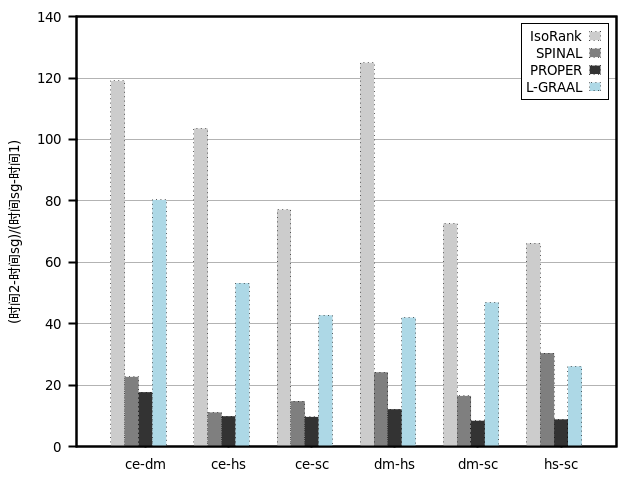
\includegraphics[height=0.25\textheight]{pic/allt-t2.png}
\caption{SGOPT与两种方案之间运行时间的对比} 
\label{fig:allt-t2}
\end{figure}

综合时间和效果的比较来看,虽然方案二的比对效果较好,但是方案二在时间上的表现实在是令人难以接受的,因此,虽然方案二的比对效果略高于SGOPT的结果,也难以被采用。而方案一虽然在运行时间上比SGOPT快,但是从实验结果中可以看到,这一点的时间优势,并不能补足其在比对效果上带来的损失。因此,SGOPT算法无论从时间上,还是比对效果上,无疑是一个更好的选择。

%@@@@@@@@@@@@@@@@@@@@@@@@@@@@@@@@@@@@@2
\section{DEC,DICS,$DS^3$,DTWEC指标的对比}
目前为止所有的实验采用的衡量指标都是CE值,那么在另外的指标下,SGOPT算法的效果又如何呢?由于方案二的指标都高于SGOPT算法,这里只针对SGOPT算法和方案一进行了实验比较。

图\ref{fig:other}是所有六组实验下,用SGOPT算法求得的各项指标,与优化前静态算法求得的比对得到的指标的对比。可以看到,SGOPT对于IsoRank的优化依旧非常明显,这是IsoRank算法效果太糟糕的缘故。而除了IsoRank,SGOPT在大部分情况下对于其他的四项指标都能产生很好的优化效果,而且和图\ref{fig:all_improve}相似的,在SPINAL和PROPER的优化上相差不多,而对于L-GRAAL的优化则相对较差。另外值得一提的便是优化呈负效果的那些情况。

\begin{figure}[htbp]
\centering
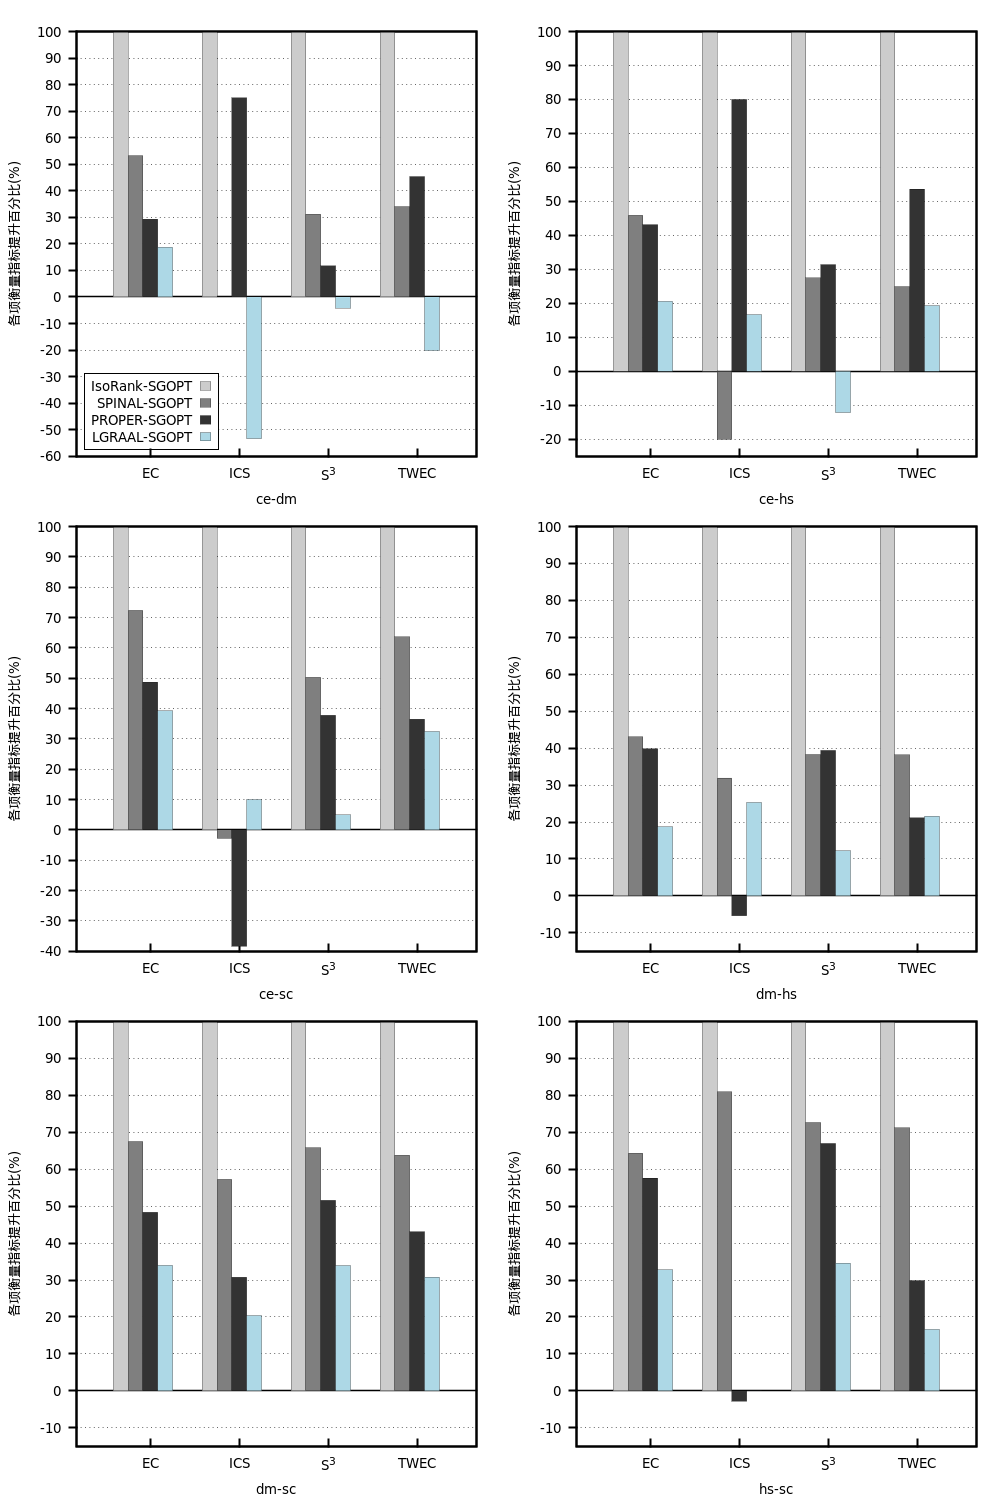
\includegraphics[width=\textwidth]{pic/other.png}
\caption{SGOPT相比其他四种算法在DEC,DICS,$DS^3$,DTWEC指标上提高的程度} 
\label{fig:other}
\end{figure}

由DEC值的定义\ref{defndec}可知,DEC值与CE值成正比关系,而由于SGOPT算法优化的便是CE值,所以在所有实验中,DEC指标相较于静态算法肯定都可以得到优化,实验也证明了这一点。

而由DICS和$DS^3$的定义\ref{defndics}, \ref{defnds3}可知,指标不仅和源网络有关,和目标网络也有关,而在目标网络是动态的情况下,优化CE值\textbf{不一定}能带动这两项指标的增长。实验也反应了这个情况,在前三组实验中,DICS在后面三种算法的优化上有时会达到负的优化效果,这样的情况出现了5次,而$DS^3$则相对较好,只出现了2次。后三组试实验中,情况则比较乐观。

理论上看,SGOPT算法的目的是优化CE值,而CE值越大,意味着源网络有更多的边被保留在了目标网络中,因此对于DEC这个只考虑源网络结构的指标,有很好的优化效果。而DICS是只考虑目标网络结构的指标,着重衡量目标网络中被匹配边的稀疏程度,而不是源网络,所以在目标网络是稠密网络的情况下,以优化CE值为目的的SGOPT算法对于这个DICS这个指标比较敏感,时好时坏。而剩下的$DS^3$和DTWEC指标,则同时考虑了源网络和目标网络,因此相对于DICS指标来说,更具有综合意义。而且SGOPT对于这两个指标的敏感程度,明显没有DICS来得高,从实验结果中也可以看到。


